\documentclass[12pt]{article}
\usepackage[danish]{babel}
\usepackage{amsfonts, amssymb, mathtools, amsthm, amsmath}
\usepackage{graphicx, pgfplots}
\usepackage{url}
\usepackage[dvipsnames]{xcolor}
\usepackage{sagetex}
\usepackage{lastpage}

%loaded last
\usepackage[hidelinks]{hyperref}

\usepackage{siunitx}
  \sisetup{exponent-product = \cdot,
    output-decimal-marker = {,}}

%Giles Castelles incfig
\usepackage{import}
\usepackage{xifthen}
\usepackage{pdfpages}
\usepackage{transparent}

\newcommand{\incfig}[2][1]{%
  \def\svgwidth{#1\columnwidth}
  \import{../figures/}{#2.pdf_tex}
}

\setlength{\parindent}{0in}
\setlength{\oddsidemargin}{0in}
\setlength{\textwidth}{6.5in}
\setlength{\textheight}{8.8in}
\setlength{\topmargin}{0in}
\setlength{\headheight}{18pt}

\usepackage{fancyhdr}
\pagestyle{fancy}

\fancyhead{}
\fancyfoot{}
\fancyfoot[R]{\thepage}
\fancyhead[C]{\leftmark}

\pgfplotsset{compat=newest}

\pgfplotsset{every axis/.append style={
  axis x line=middle,    % put the x axis in the middle
  axis y line=middle,    % put the y axis in the middle
  axis line style={<->,color=black}, % arrows on the axis
}}

\usepackage{thmtools}
\usepackage{tcolorbox}
  \tcbuselibrary{skins, breakable}
  \tcbset{
    space to upper=1em,
    space to lower=1em,
  }

\theoremstyle{definition}

\newtcolorbox[auto counter]{definition}[1][]{%
  breakable,
  colframe=ForestGreen,  %frame color
  colback=ForestGreen!5, %background color
  colbacktitle=ForestGreen!25, %background color for title
  coltitle=ForestGreen!70!black,  %title color
  fonttitle=\bfseries\sffamily, %title font
  left=1em,              %space on left side in box,
  enhanced,              %more options
  frame hidden,          %hide frame
  borderline west={2pt}{0pt}{ForestGreen},  %display left line
  title=Definition \thetcbcounter: #1,
}

\newtcolorbox{greenline}{%
  breakable,
  colframe=ForestGreen,  %frame color
  colback=white,          %remove background color
  left=1em,              %space on left side in box
  enhanced,              %more options
  frame hidden,          %hide frame
  borderline west={2pt}{0pt}{ForestGreen},  %display left line
}

\newtcolorbox[auto counter, number within=section]{eks}[1][]{%
  brekable,
  colframe=NavyBlue,  %frame color
  colback=NavyBlue!5, %background color
  colbacktitle=NavyBlue!25,    %background color for title
  coltitle=NavyBlue!70!black,  %title color
  fonttitle=\bfseries\sffamily, %title font
  left=1em,            %space on left side in box,
  enhanced,            %more options
  frame hidden,        %hide frame
  borderline west={2pt}{0pt}{NavyBlue},  %display left line
  title=Eksempel \thetcbcounter: #1
}

\newtcolorbox{blueline}{%
  breakable,
  colframe=NavyBlue,     %frame color
  colback=white,         %remove background
  left=1em,              %space on left side in box,
  enhanced,              %more options
  frame hidden,          %hide frame
  borderline west={2pt}{0pt}{NavyBlue},  %display left line
}

\newtcolorbox{teo}[1][]{%
  breakable,
  colframe=RawSienna,  %frame color
  colback=RawSienna!5, %background color
  colbacktitle=RawSienna!25,    %background color for title
  coltitle=RawSienna!70!black,  %title color
  fonttitle=\bfseries\sffamily, %title font
  left=1em,              %space on left side in box,
  enhanced,              %more options
  frame hidden,          %hide frame
  borderline west={2pt}{0pt}{RawSienna},  %display left line
  title=Teori: #1,
}

\newtcolorbox[auto counter, number within=section]{sæt}[1][]{%
  breakable,
  colframe=RawSienna,  %frame color
  colback=RawSienna!5, %background color
  colbacktitle=RawSienna!25,    %background color for title
  coltitle=RawSienna!70!black,  %title color
  fonttitle=\bfseries\sffamily, %title font
  left=1em,              %space on left side in box,
  enhanced,              %more options
  frame hidden,          %hide frame
  borderline west={2pt}{0pt}{RawSienna},  %display left line
  title=Sætning \thetcbcounter: #1,
  before lower={\textbf{Bevis:}\par\vspace{0.5em}},
  colbacklower=RawSienna!25,
}

\newtcolorbox{redline}{%
  breakable,
  colframe=RawSienna,  %frame color
  colback=white,       %Remove background color
  left=1em,            %space on left side in box,
  enhanced,            %more options
  frame hidden,        %hide frame
  borderline west={2pt}{0pt}{RawSienna},  %display left line
}

\newtcolorbox{for}[1][]{%
  breakable,
  colframe=NavyBlue,  %frame color
  colback=NavyBlue!5, %background color
  colbacktitle=NavyBlue!25,    %background color for title
  coltitle=NavyBlue!70!black,  %title color
  fonttitle=\bfseries\sffamily, %title font
  left=1em,              %space on left side in box,
  enhanced,              %more options
  frame hidden,          %hide frame
  borderline west={2pt}{0pt}{NavyBlue},  %display left line
  title=Forklaring #1,
}

\newtcolorbox{bem}{%
  breakable,
  colframe=NavyBlue,  %frame color
  colback=NavyBlue!5, %background color
  colbacktitle=NavyBlue!25,    %background color for title
  coltitle=NavyBlue!70!black,  %title color
  fonttitle=\bfseries\sffamily, %title font
  left=1em,              %space on left side in box,
  enhanced,              %more options
  frame hidden,          %hide frame
  borderline west={2pt}{0pt}{NavyBlue},  %display left line
  title=Bemærkning:,
}

\makeatother
\def\@lecture{}%
\newcommand{\lecture}[3]{
  \ifthenelse{\isempty{#3}}{%
    \def\@lecture{Lecture #1}%
  }{%
    \def\@lecture{Lecture #1: #3}%
  }%
  \subsection*{\makebox[\textwidth][l]{\@lecture \hfill \normalfont\small\textsf{#2}}}
}

\makeatletter

\newcommand{\opgave}[1]{%
 \def\@opgave{#1}%
 \subsection*{Opgave #1}
}

\makeatother

%Format lim the same way in intext and in display
\let\svlim\lim\def\lim{\svlim\limits}

% horizontal rule
\newcommand\hr{
\noindent\rule[0.5ex]{\linewidth}{0.5pt}
}

\title{Opgaver til forelæsning uge 23}
\author{Noah Rahbek Bigum Hansen}
\date{26. November 2024}

\begin{document}

\maketitle

\section*{Opg. 12.1}
On a part-time job, you are asked to bring a cylindrical iron rod of length \qty{85,8}{cm} and diameter \qty{2,85}{cm} from a storage room to a machinist. Will you need a cart? (To answer, calculate the weight of the rod.)
\bigbreak
Først findes volumenet af stangen vha. formlen for volumenet af en cylinder som
\[ 
V = \pi \cdot h\cdot r^2 = \pi \cdot \left( \frac{\qty{2,85}{cm}}{2} \right)^2 \cdot \qty{85,8}{cm} = \qty{5,473e-4}{m^3} 
.\]
Og dermed kan massen af stangen findes vha. densiteten for jern $\rho = \qty{7,8e3}{\frac{kg}{m^3}}$ som
\[ 
m = \rho \cdot V = \qty{7,8e3}{\frac{kg}{m^3}} \cdot \qty{5,473e-4}{m^3} = \qty{4,27}{kg} 
.\]
Altså behøver jeg ikke en vogn, fordi jeg er en stærk dreng, der godt kan løfte \qty{4,27}{kg}.



\section*{Opg. 12.5}
A uniform lead sphere and a uniform aluminum sphere have the same mass. What is the ratio of the radius of the aluminum sphere to the radius of the lead sphere?
\bigbreak
Idet vi har at
\[ 
m \sim r^3
.\]
For de to sfærer har vi at
\begin{align*}
  \rho_l \cdot r_l^3 &= \rho_a \cdot r_a^3 \\
  \frac{r_a}{r_l} &= \sqrt[3]{\frac{\rho_l}{\rho_a}} \\
                  &= \sqrt[3]{\frac{\qty{11,3e3}{\frac{kg}{m^3}}}{\qty{2,7e3}{\frac{kg}{m^3}} }} \\
                  &= \num{1,612}  
.\end{align*}
Altså skal en kugle af aluminium have en radius, der er omkring 60\% større end en kugle med bly for at de to kugler får samme masse.

\section*{Opg. 12.19}
\begin{figure} [ht]
  \centering
  \caption{}
  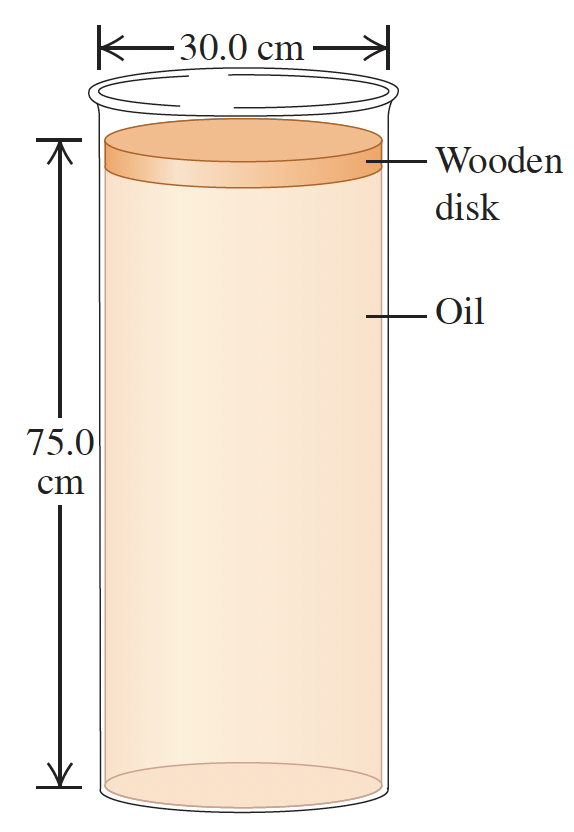
\includegraphics[width=0.3\linewidth]{../figures/F23_12_19.png}
  \label{fig:F23_12_19}
\end{figure}
A cylindrical disk of wood weighing \qty{45,0}{N} and having a diameter of \qty{30,0}{cm} floats on a cylinder of oil of density \qty{0,850}{g/cm^3} (\textbf{\autoref{fig:F23_12_19}}). The cylinder of oil is \qty{75,0}{cm}  deep and has a diameter the same as that of the wood.

\subsection*{(a)}
What is the gauge pressure at the top of the oil column?
\bigbreak
Generelt er tryk givet som
\[ 
p = \frac{F}{A}
.\]
Sættes tallene fra opgaven ind fås
\[ 
p_0 = \frac{\qty{45,0}{N}}{\pi \cdot \left( \frac{\qty{30,0}{cm}}{2} \right)^2} = \qty{637}{Pa} 
.\]

\subsection*{(b)}
Suppose now that someone puts a weight of \qty{83,0}{N} on top of the wood, but no oil seeps around the edge of the wood. What is the change in pressure at

\subsubsection*{(i)}
the bottom of the oil and
\bigbreak
Ændringen i trykket findes som i opgaven ovenfor som
\[ 
\Delta p = \frac{\qty{83,0}{N}}{\pi \cdot \left( \qty{15,0}{cm}  \right)^2} = \qty{1174}{Pa} 
.\]


\subsubsection*{(ii)}
halfway down in the oil?
\bigbreak
Her er svaret som ovenfor, da det tilføjede tryk vil fordele sig ens igennem hele væsken. 


\section*{Opg. 12.33}
\begin{figure} [ht]
  \centering
  \caption{}
  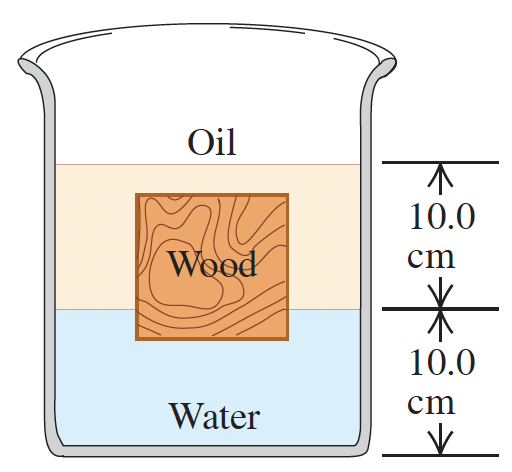
\includegraphics[width=0.3\linewidth]{../figures/F23_12_33.png}
  \label{fig:F23_12_33}
\end{figure}
A cubical block of wood, \qty{10,0}{cm} on a side, floats at the interface between oil and water with its lower surface \qty{1,50}{cm} below the interface
(\textbf{\autoref{fig:F23_12_33}}). The density of the oil is \qty{790}{kg/m^3}.

\subsection*{(a)}
What is the gauge pressure at the upper face of the block?
\bigbreak
Trykket $p$ kan findes ud fra formlen for tryk
\[ 
p = \rho \cdot g \cdot h = \qty{790}{\frac{kg}{m^3}} \cdot \qty{9,80}{\frac{m}{s^2}} \cdot \qty{1,50}{cm} = \qty{116}{Pa}
.\]

\subsection*{(b)}
What is the gauge pressure at the lower face of the block?
\bigbreak
Først findes trykket ved grænsefladen mellem olie og vand som
\[ 
p_{ov} = \qty{790}{\frac{kg}{m^3}} \cdot \qty{9,80}{\frac{m}{s^2}} \cdot \qty{10}{cm} = \qty{774,2}{Pa} 
.\]
Og trykket fra vandet kan da findes som
\[ 
p_{v} = \qty{1000}{\frac{kg}{m^3}} \cdot \qty{9,80}{\frac{m}{s^2}} \cdot \qty{1,50}{cm} \qty{147}{Pa} 
.\]
Altså er det samlede \textit{gauge-pressure} ved bunden af blokken givet som
\[ 
  p_{b} = p_{ov} + p_2 = \qty{116}{Pa} + \qty{774,2}{Pa} + \qty{147}{Pa} = \qty{921}{Pa}
.\]


\subsection*{(c)}
What are the mass and density of the block?
\bigbreak
Først findes volumenet af blokken indeholdt i hhv. vandet og olien som
\begin{align*}
  V_o &= \qty{10}{cm} \cdot \qty{10}{cm} \cdot \qty{8.5}{cm} = \qty{8.5e-4}{m^3} \\
  V_v &= \qty{10}{cm} \cdot \qty{10}{cm} \cdot \qty{1.5}{cm} = \qty{1.5e-4}{m^3} 
.\end{align*}
Opdrift er generelt givet som
\[ 
F_{op} = \rho \cdot V \cdot g
.\]
Vi har altså en samlet opdrift på
\[ 
F_{op} = g(\rho_o \cdot V_o + \rho_v \cdot V_v) = \qty{9.80}{\frac{m}{s^2}} \cdot (\qty{790}{\frac{kg}{m^3}} \cdot \qty{8.5e-4}{m^3} + \qty{1000}{\frac{kg}{m^3}} \cdot \qty{1.5e-4}{m^3}) = \qty{8.05}{N}  
.\]
Idet der er statisk ligevægt må det gælde at
\[ 
F_{op} = F_g = \qty{8.05}{N} 
.\]
Altså er massen af blokken
\[ 
m = \frac{F}{g} = \frac{\qty{8.05}{N}}{\qty{9.80}{\frac{m}{s^2}}} = \qty{0.821}{kg} 
.\]
Og blokkens densitet bliver da
\[ 
\rho =  \frac{m}{V} = \frac{\qty{0.821}{kg}}{\left( \qty{0.10}{m} \right)^3} = \qty{821}{\frac{kg}{m^3}} 
.\]


\section*{Opg. 12.35}
A rock is suspended by a light string. When the rock is in air, the tension in the string is \qty{39,2}{N}. When the rock is totally immersed in water, the tension is \qty{28,4}{N}. When the rock is totally immersed in an unknown liquid, the tension is \qty{21,5}{N}. What is the density of the unknown liquid?
\bigbreak
Først findes massen af stenen som
\[ 
m = \frac{F_g}{g} = \frac{\qty{39,2}{N}}{\qty{9,80}{\frac{m}{s^2}}} = \qty{4,00}{kg} 
.\]
Idet stenen nedsænkes i vandet falder den effektive tænkte med en værdi tilsvarende opdriften på blokken $F_{op} = T_0 - T_1 = \qty{39,2}{N} - \qty{28,4}{N} = \qty{10,8}{N}$. Formlen for opdrift kan nu bruges til at finde volumenet af stenen som
\[ 
F_{op} = \rho Vg \implies V = \frac{F_{op}}{\rho \cdot g} = \frac{\qty{10,8}{N}}{\qty{1000}{\frac{kg}{m^3}} \cdot \qty{9,80}{\frac{m}{s^2}}} = \qty{0.0011}{m^3} 
.\]
Idet stenen nedsænkes i den ukendte væske får den en opdrift på $F_{op_2} = \qty{39,2}{N} - \qty{21,5}{N} = \qty{17,7}{N}$. Vi kan da finde densiteten af den ukendte væske som
\[ 
\rho = \frac{F_{op_2}}{Vg} = \frac{\qty{17,7}{N}}{\qty{0.0011}{m^3} \cdot \qty{9.8}{\frac{m}{s^2}}} = \qty{1641.9}{\frac{kg}{m^3}} 
.\]



\section*{Opg. 12.55}
A swimming pool is \qty{5,0}{m} long, \qty{4,0}{m} wide, and \qty{3,0}{m} deep. Compute the force exerted by the water against

\subsection*{(a)}
the bottom
\bigbreak
Trykket på bunden er givet ved den almindelige trykformel som
\[ 
p_{b} = \rho \cdot g \cdot h = \qty{1000}{\frac{kg}{m^3}} \cdot \qty{9.80}{\frac{m}{s^2}} \cdot \qty{3,00}{m} = \qty{2,94e4}{Pa}
.\]
Og kraften på bunden bliver da
\[ 
F_{b} = p_b \cdot A = \qty{29400}{Pa} \cdot \qty{5.0}{m} \cdot \qty{4.0}{m} = \qty{5,88e5}{N} 
.\]


\subsection*{(b)}
either end. (\textit{Hint:} Calculate the force exerted on a thin, horizontal strip at a depth $h$, and integrate this over the end of the pool.) Do not include the force due to air pressure.
\bigbreak
Vha. formlen for tryk kan trykket på en tynd stribe som funktion af højden opstilles som
\[ 
p(h) = \rho \cdot g \cdot h 
.\]
Kraften bliver da
\[ 
F(h) = b \cdot \rho \cdot g \cdot h
.\]
Denne kraft kan integreres over hele højden for at få
\begin{align*}
  F &= b \cdot \rho \cdot g \int_{\qty{0}{m}}^{\qty{3,00}{m}} h \, \mathrm{d}h \\
  &= \qty{4,00}{m} \cdot \qty{1000}{\frac{kg}{m^3}} \cdot \qty{9.80}{\frac{m}{s^2}} \cdot \frac{1}{2}\cdot (\qty{3,00}{m})^2 \\
  &= \qty{1,76e5}{N} 
.\end{align*}


\section*{Opg. 12.65}
A large, \qty{40,0}{kg} cubical block of wood with uniform density is floating in a freshwater lake with \num{20,0}\% of its volume above the surface of the water. You want to load bricks onto the floating block and then push it horizontally through the water to an island where you are building an outdoor grill.

\subsection*{(a)}
What is the volume of the block?
\bigbreak
Vi opskriver flydeligevægten som
\begin{align*}
  F_b &= F_g \\
  \num{0.8} V \rho g &= mg \\
  V &= \frac{m}{\num{0.8} \rho} \\
    &= \frac{\qty{40,0}{kg}}{\num{0.8} \cdot \qty{1000}{\frac{kg}{m^3}}} = \qty{5,00e-2}{m^3} 
.\end{align*}


\subsection*{(b)}
What is the maximum mass of bricks that you can place on the block without causing it to sink below the water surface?
\bigbreak
Vi kan igen opskrive ligevægten fra før dog med en ekstra masse denne gang så vi får at
\begin{align*}
  (m + M)g &= V \rho g \\
  m + M &= V \rho g \\
  M &= V \rho - m \\
    &= \qty{5,00e-2}{m^3} \cdot \qty{1000}{\frac{kg}{m^3}} - \qty{40,0}{kg} \\ 
    &= \qty{10}{kg} 
.\end{align*}


\section*{Opg. 12.72}
\begin{figure} [ht]
  \centering
  \caption{}
  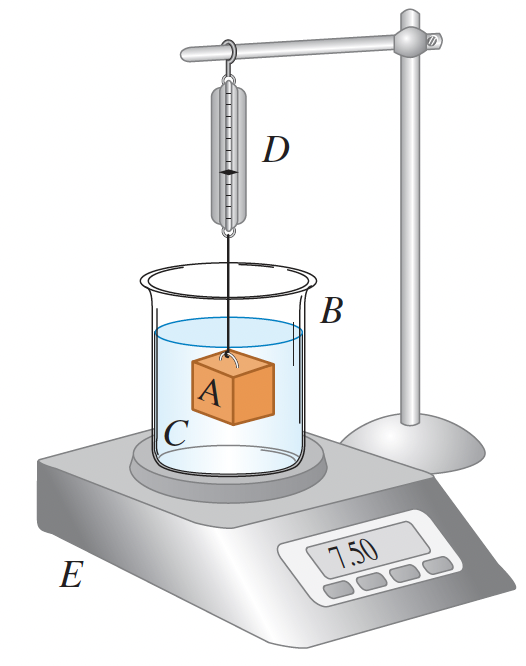
\includegraphics[width=0.3\linewidth]{../figures/F23_12_72.png}
  \label{fig:F23_12_72}
\end{figure}

Block $A$ in \textbf{\autoref{fig:F23_12_72}} hangs by a cord from spring balance $D$ and is submerged in a liquid $C$ contained in beaker $B$. The mass of the beaker is \qty{1,00}{kg}; the mass of the liquid is \qty{1,80}{kg}. Balance $D$ reads \qty{3,50}{kg}, and balance $E$ reads \qty{7,50}{kg}. The volume of the block $A$ is \qty{3,80e-3}{m^3}.

\subsection*{(a)}
What is the density of the liquid?

\subsection*{(b)}
What will each balance read if block $A$ is pulled up out of the liquid. 

\end{document}
